% CMP6232 Assessment 2 — Final Report
% Build: pdflatex main && bibtex main && pdflatex main && pdflatex main
% On Overleaf: upload the three PNGs from results/figures/ and the Python
% files referenced in the appendix, adjusting the ../ paths.
\documentclass[11pt,a4paper]{article}

\usepackage[margin=2.5cm]{geometry}
\usepackage{booktabs}
\usepackage{multirow}
\usepackage{graphicx}
\usepackage[round]{natbib}
\usepackage{listings}
\usepackage{xcolor}
\usepackage[hidelinks]{hyperref}

\graphicspath{{../results/figures/}}

\lstset{
  language=Python, basicstyle=\ttfamily\scriptsize, breaklines=true,
  commentstyle=\color{gray}, keywordstyle=\bfseries,
  frame=single, numbers=left, numberstyle=\tiny\color{gray},
  showstringspaces=false,
}

\title{Parameter-Efficient Fine-Tuning for Nepali:\\
LoRA vs.\ Full Fine-Tuning Across Three NLUE Tasks}
\author{Subresh Thakulla\\Student ID: XXXXXXXX} % TODO: insert student ID
\date{August 2026}

\begin{document}
\maketitle

\begin{abstract}
This report compares full fine-tuning with Low-Rank Adaptation (LoRA)
across four pre-trained encoders --- two monolingual Nepali models
(NepBERTa, IRIIS-RoBERTa) and two multilingual models (mBERT, XLM-R base)
--- on three Nepali language-understanding tasks of decreasing size:
sentiment analysis (65\,k examples), linguistic acceptability (7.8\,k),
and coreference resolution (564). Across a 78-run grid on free-tier GPU
hardware, three findings emerge. First, on the two larger tasks full
fine-tuning is consistently best, but LoRA trails by only 3--8 macro-F1
points while training under 1\,\% of the parameters at roughly half the
memory and time. Second, at 564 examples the ordering inverts: full
fine-tuning collapses to majority-class prediction on every model, while
LoRA degrades gracefully and wins on all four; a rank ablation is
consistent with adapter capacity, not the adaptation method, being the
risk factor. Third, tokenizer fertility varies $2.3\times$ across the
models and tracks downstream quality and cost better than the
monolingual/multilingual distinction does, making vocabulary quality a
first-order model-selection criterion for Nepali.
\end{abstract}

\section{Introduction}
\label{sec:intro}

Nepali is spoken by over 30 million people yet remains low-resourced in
NLP: labelled datasets are small, and practitioners typically cannot
afford the hardware that modern fine-tuning assumes. Parameter-efficient
fine-tuning (PEFT) methods --- adapters \citep{houlsby2019adapters}, LoRA
\citep{hu2022lora}, and quantised variants such as QLoRA
\citep{dettmers2023qlora} --- promise near-full-fine-tuning quality at a
fraction of the compute, but the evidence base is overwhelmingly
English-centric. Whether these trade-offs hold for a morphologically rich,
Devanagari-script language, across both monolingual and multilingual
pre-trained models, is an open practical question.

The aim of this report is to quantify that trade-off for Nepali. Using
three publicly released classification tasks from the NLUE benchmark
\citep{nyachhyon2025nlue} --- sentiment analysis, linguistic
acceptability, and coreference resolution, spanning three orders of
magnitude in training-set size --- it evaluates full fine-tuning against
LoRA on four pre-trained encoders under a fixed, method-fair training
budget. The main achievements are: (i) a complete, reproducible 78-run
experimental grid executed entirely on free-tier GPU hardware; (ii) a
quantified accuracy--efficiency trade-off for LoRA in Nepali, including a
data-scarcity regime in which LoRA \emph{outperforms} full fine-tuning;
and (iii) a tokenizer-fertility analysis linking vocabulary quality to
both accuracy and cost.

The report is organised as follows. Section~\ref{sec:problem} describes
the datasets and formalises the problem. Section~\ref{sec:method} details
the models, pre-processing, and adaptation methods.
Section~\ref{sec:results} presents parameter settings, the evaluation
process, and results. Section~\ref{sec:summary} discusses the findings,
and the appendix lists the Python code used to build and evaluate the
models.

\section{Problem Statement}
\label{sec:problem}

The task is supervised text classification for Nepali under realistic
resource constraints. Three binary classification datasets are drawn from
the NLUE benchmark \citep{nyachhyon2025nlue}, all released as
Hugging Face datasets with train/test splits:

\begin{description}
  \item[Sentiment analysis] (65{,}106 train / 16{,}279 test): single
  sentences labelled positive or negative.
  \item[Linguistic acceptability] (7{,}799 / 1{,}950): a Nepali analogue
  of the Corpus of Linguistic Acceptability \citep{warstadt2019cola};
  single sentences labelled grammatically acceptable or not.
  \item[Coreference resolution] (564 / 142): sentence pairs, cast as
  binary classification of whether the marked mentions corefer.
\end{description}

The spread in size --- roughly $115\times$ between the largest and
smallest training set --- is deliberate: it turns dataset scale into an
experimental axis. The deep learning problem is then a controlled
$4 \times 2$ comparison: four pre-trained transformer encoders (two
monolingual Nepali, two multilingual) crossed with two adaptation methods
(full fine-tuning vs.\ LoRA), asking (a) how much accuracy LoRA concedes
at each data scale, (b) what it saves in memory, time, and storage, and
(c) whether pre-training language or tokenizer quality better predicts
downstream performance.

\section{Proposed Method}
\label{sec:method}

\subsection{Models}

Four publicly available encoders are compared
(Table~\ref{tab:models}): NepBERTa \citep{timilsina2022nepberta} and
IRIIS-RoBERTa \citep{iriisroberta2024} are monolingual Nepali models;
mBERT \citep{devlin2019bert} and XLM-R base \citep{conneau2020xlmr} are
multilingual. All are BERT-family encoders at the 110--280M-parameter
scale, so the comparison isolates pre-training data and vocabulary rather
than architecture. NepBERTa is distributed as TensorFlow weights only;
the checkpoint was converted to PyTorch once, verified against the
original, and re-published so that all runs share one framework.
Each model's true parameter and vocabulary counts were verified
programmatically before the campaign.

\begin{table}[t]
  \centering
  \caption{Verified model checkpoints.}
  \label{tab:models}
  \begin{tabular}{llrr}
    \toprule
    Model & Family & Params & Vocab \\
    \midrule
    NepBERTa      & monolingual  & 109.5\,M & 30{,}523 \\
    IRIIS-RoBERTa & monolingual  & 124.6\,M & 50{,}256 \\
    mBERT         & multilingual & 177.9\,M & 119{,}547 \\
    XLM-R base    & multilingual & 278.0\,M & 250{,}002 \\
    \bottomrule
  \end{tabular}
\end{table}

\subsection{Pre-processing}

Each dataset is loaded from its canonical repository and tokenized with
the corresponding model's subword tokenizer (maximum length 128 tokens
for the single-sentence tasks, 256 for coreference sentence pairs, which
are encoded jointly with the standard pair template). Labels are cast to
categorical form, and dynamic padding is applied per batch. Because the
released datasets ship without validation splits, a stratified 10\,\% of
each training set is held out as validation using a \emph{fixed} split
seed, separate from the training seed: every run in the grid sees the
identical train/validation partition, so cross-condition comparisons are
not confounded by partition noise. Only training randomness
(initialisation, shuffling, dropout) varies with the per-run seed.

\subsection{Adaptation methods}

\textbf{Full fine-tuning} updates all encoder weights plus a randomly
initialised classification head. \textbf{LoRA} \citep{hu2022lora} freezes
the encoder and injects trainable low-rank matrices $BA$ (rank $r$,
scaling $\alpha = 2r$) into the attention query and value projections,
following the original paper; the classification head remains trainable.
At the default $r{=}8$ this trains 887{,}042 parameters --- between
0.32\,\% and 0.80\,\% of each model. LoRA is implemented with the PEFT
library \citep{mangrulkar2022peft} on Hugging Face Transformers
\citep{wolf2020transformers}. A rank ablation on the smallest task varies
$r \in \{4, 8, 16, 32\}$ to separate the effect of adapter capacity from
the method itself. Complementing the accuracy comparison, tokenizer
\emph{fertility} (mean subword tokens per whitespace word) is measured
for all four models on the acceptability test set.

% Section 4 (Experimental Results) and Section 5 (Summary)
% Results and Discussion sections — CMP6232 Assessment 2
% Requires: \usepackage{booktabs} \usepackage{multirow} \usepackage{graphicx}
% Figures referenced from results/figures/ — adjust \graphicspath as needed:
% \graphicspath{{../results/figures/}}

\section{Experimental Results}
\label{sec:results}

\subsection{Parameter settings and evaluation process}
\label{sec:params}

Every run is defined by one YAML configuration and appends one row to a
results log, giving a fully scripted, resumable 78-run campaign. Within a
task, epochs, batch size, and maximum sequence length are identical across
methods and models (Table~\ref{tab:params}); only the learning rate differs
by method, set to each method's published standard --- $2\times10^{-5}$ for
full fine-tuning and $2\times10^{-4}$ for LoRA \citep{hu2022lora}. Training
uses the AdamW optimiser \citep{loshchilov2019adamw} with mixed precision
(fp16) via the Hugging Face \texttt{Trainer} \citep{wolf2020transformers}.
The model is evaluated on the validation split after every epoch, and the
checkpoint with the best validation macro-F1 is restored before the single,
final test-set evaluation. Macro-F1 is the primary metric (both label
distributions are imbalanced); accuracy is reported alongside, and Matthews
correlation (MCC) additionally for acceptability, following
\citet{warstadt2019cola}. Peak GPU memory and wall-clock minutes are
recorded per run.

\begin{table}[t]
  \centering
  \caption{Fixed per-task training budget (identical across methods and
  models). Learning rate is the only method-specific setting; LoRA uses
  $\alpha = 2r$ throughout.}
  \label{tab:params}
  \begin{tabular}{lccc}
    \toprule
    & Sentiment & Acceptability & Coreference \\
    \midrule
    Epochs          & 3   & 5   & 15  \\
    Batch size      & 32  & 32  & 16  \\
    Max length      & 128 & 128 & 256 \\
    \bottomrule
  \end{tabular}
\end{table}

\subsection{Main results}

All results are reported as test macro-F1, averaged over three random seeds
(42--44) with standard deviation (except the rank ablation at
$r \in \{4, 16, 32\}$, which uses two seeds); the train/validation partition is fixed
across every run so that cross-condition comparisons are valid.
LoRA uses rank
$r{=}8$ unless stated otherwise, training 887\,k parameters
(0.32--0.80\,\% of each model) against 109--278\,M for full fine-tuning.
Table~\ref{tab:main} summarises the full grid; Figure~\ref{fig:pareto} plots
the accuracy--capacity trade-off.

\begin{table}[t]
  \centering
  \caption{Test macro-F1 (mean $\pm$ std over 3 seeds) for full fine-tuning
  (Full) and LoRA ($r{=}8$). $\Delta$ = Full $-$ LoRA; negative values mean
  LoRA wins. For acceptability, Matthews correlation (MCC) is given in
  parentheses.}
  \label{tab:main}
  \begin{tabular}{llccc}
    \toprule
    Task & Model & Full & LoRA & $\Delta$ \\
    \midrule
    \multirow{4}{*}{Sentiment (65\,k)}
      & XLM-R base      & $.881 \pm .001$ & $.852 \pm .001$ & $+.029$ \\
      & IRIIS-RoBERTa   & $.878 \pm .001$ & $.850 \pm .001$ & $+.028$ \\
      & NepBERTa        & $.867 \pm .002$ & $.821 \pm .002$ & $+.047$ \\
      & mBERT           & $.864 \pm .000$ & $.808 \pm .001$ & $+.056$ \\
    \midrule
    \multirow{4}{*}{Acceptability (7.8\,k)}
      & IRIIS-RoBERTa   & $.812 \pm .006$ \,(.648) & $.765 \pm .004$ \,(.580) & $+.047$ \\
      & XLM-R base      & $.808 \pm .012$ \,(.630) & $.730 \pm .007$ \,(.520) & $+.077$ \\
      & NepBERTa        & $.806 \pm .003$ \,(.626) & $.737 \pm .003$ \,(.510) & $+.069$ \\
      & mBERT           & $.769 \pm .005$ \,(.554) & $.721 \pm .006$ \,(.494) & $+.048$ \\
    \midrule
    \multirow{4}{*}{Coreference (564)}
      & mBERT           & $.327 \pm .017$ & $.413 \pm .017$ & $-.085$ \\
      & NepBERTa        & $.329 \pm .023$ & $.408 \pm .021$ & $-.079$ \\
      & IRIIS-RoBERTa   & $.307 \pm .027$ & $.382 \pm .046$ & $-.075$ \\
      & XLM-R base      & $.317 \pm .000$ & $.354 \pm .070$ & $-.036$ \\
    \bottomrule
  \end{tabular}
\end{table}

\begin{figure}[t]
  \centering
  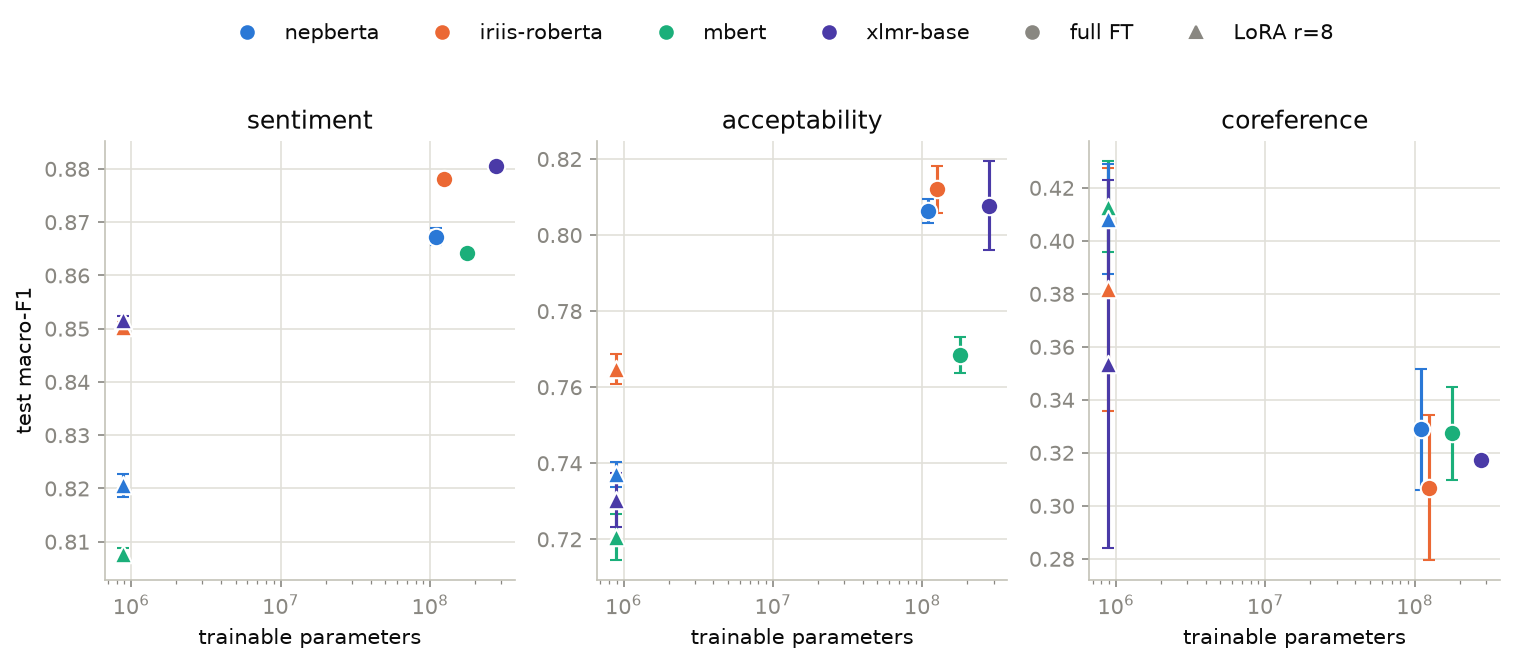
\includegraphics[width=\linewidth]{pareto.png}
  \caption{Test macro-F1 against trainable parameters (log scale), one panel
  per task. Circles = full fine-tuning, triangles = LoRA $r{=}8$; error bars
  span $\pm 1$ std over seeds. On the two larger tasks full fine-tuning
  dominates; on the 564-example coreference task the ordering inverts.}
  \label{fig:pareto}
\end{figure}

\subsection{Sentiment and acceptability: full fine-tuning wins, LoRA stays close}

On sentiment, the largest task, full fine-tuning is best for every model,
led by XLM-R base ($.881$) and IRIIS-RoBERTa ($.878$). LoRA trails by
2.8--5.6 F1 points while updating under 1\,\% of the parameters. Seed
variance is negligible throughout ($\sigma \le .002$), so these gaps,
though small, are systematic rather than noise. Acceptability shows the same
ordering with a wider LoRA gap (4.7--7.7 points; 6.0--11.6 MCC points),
consistent with the smaller training set giving the adapters fewer examples
from which to compensate for the frozen backbone.

\subsection{Coreference: full fine-tuning collapses, LoRA degrades gracefully}

With only 564 training examples, no configuration learns the task well
(macro-F1 $.31$--$.41$), but the \emph{failure modes} differ sharply. Full
fine-tuning collapses to the majority class: XLM-R full scores
$.317 \pm .000$ --- an identical, degenerate output on all three seeds. The
scores match all-one-class prediction exactly: a constant binary predictor
with accuracy $a$ has macro-F1 $a/(1+a)$, and $.4648/1.4648 = .3173$. LoRA, by contrast,
beats full fine-tuning on \emph{all four} models (by 3.6--8.5 points),
retaining some class-discriminative signal at the price of high seed variance
(up to $\sigma{=}.070$). The frozen backbone appears to act as a regulariser:
with only 887\,k free parameters, the model cannot fully re-organise its
representation around the majority-class shortcut.

\begin{figure}[t]
  \centering
  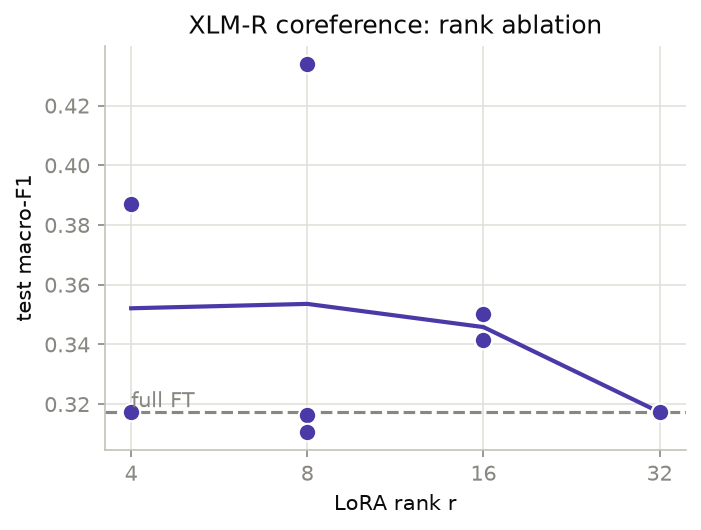
\includegraphics[width=.6\linewidth]{rank_ablation.png}
  \caption{LoRA rank ablation on XLM-R coreference. Mean test macro-F1
  is flat from $r{=}4$ to $r{=}8$ and falls thereafter; at $r{=}32$ both
  seeds land exactly on the majority-class floor reached by full
  fine-tuning (dashed line). Ranks other than 8 use two seeds.}
  \label{fig:ablation}
\end{figure}

The rank ablation (Figure~\ref{fig:ablation}) is consistent with a capacity
effect: as adapter capacity grows from $r{=}4$ to $r{=}32$
(740\,k\,$\to$\,1.77\,M trainable parameters), mean macro-F1 is flat from
$r{=}4$ to $r{=}8$ and then falls
($.352 \to .354 \to .346 \to .317$), and at $r{=}32$ the model
reproduces the full fine-tuning collapse exactly ($.317 \pm .000$). The
differences among $r \le 16$ sit within seed noise (individual seeds range
$.31$--$.43$, and one $r{=}4$ seed already lands on the collapse floor), so
the solid observation is the endpoint: at $r{=}32$, added capacity
reproduces the failure mode of full fine-tuning on data this scarce.

\subsection{Training cost}

\begin{figure}[t]
  \centering
  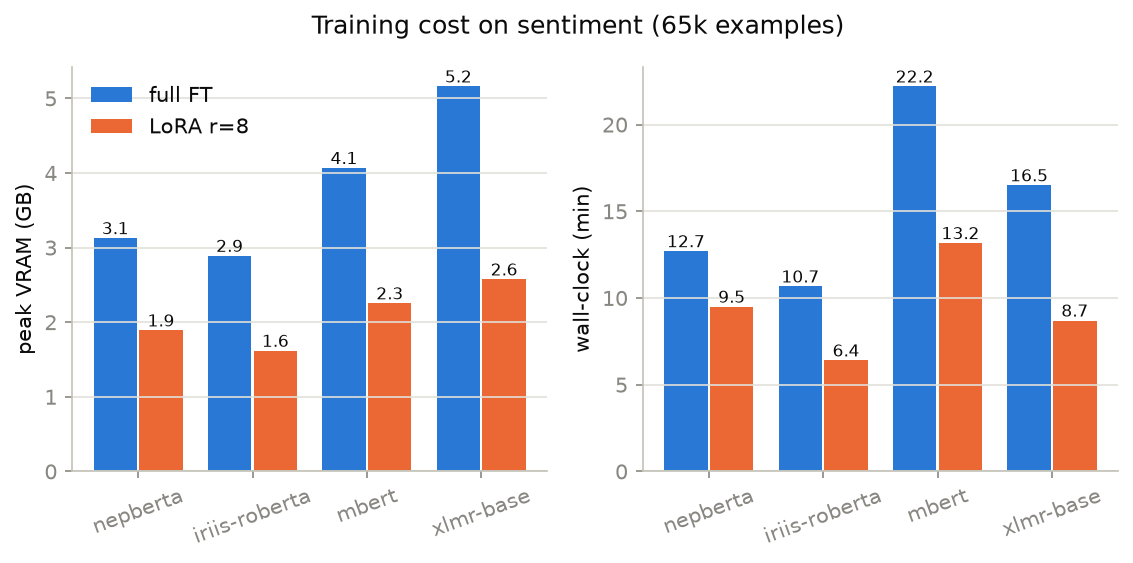
\includegraphics[width=\linewidth]{efficiency.png}
  \caption{Peak GPU memory and wall-clock time on the sentiment task
  (65\,k examples), full fine-tuning vs LoRA $r{=}8$, single T4 GPU.}
  \label{fig:efficiency}
\end{figure}

LoRA cuts peak GPU memory by 40--50\,\% (XLM-R: 5.2\,$\to$\,2.6\,GB) and
wall-clock time by 25--50\,\% on sentiment (Figure~\ref{fig:efficiency}),
with every configuration fitting comfortably on a free-tier 16\,GB T4. The
practical consequence for low-resource settings is direct: the entire
78-run study was executed on free Colab sessions, and the LoRA
checkpoints are megabytes rather than gigabytes.

\subsection{Tokenizer fertility}

\begin{table}[t]
  \centering
  \caption{Tokenizer fertility (mean subword tokens per whitespace word) on
  the 1,950-sentence acceptability test set. Lower is better.}
  \label{tab:fertility}
  \begin{tabular}{llrr}
    \toprule
    Model & Family & Vocab & Fertility \\
    \midrule
    IRIIS-RoBERTa & monolingual  & 50\,k  & 1.34 \\
    XLM-R base    & multilingual & 250\,k & 1.92 \\
    NepBERTa      & monolingual  & 30\,k  & 2.03 \\
    mBERT         & multilingual & 119\,k & 3.04 \\
    \bottomrule
  \end{tabular}
\end{table}

Fertility (Table~\ref{tab:fertility}) varies by a factor of 2.3 across the
four models. IRIIS-RoBERTa's Nepali-specific 50\,k vocabulary is the most
compact (1.34 tokens per word); mBERT fragments the average Nepali word into
more than three pieces. Notably, XLM-R's 250\,k multilingual vocabulary
achieves near-monolingual fertility (1.92), while NepBERTa's small 30\,k
Nepali vocabulary does not (2.03).

\section{Summary}
\label{sec:summary}

\paragraph{Is LoRA a viable substitute for full fine-tuning in Nepali?}
For the data regimes that matter in practice, yes, with a quantified cost.
At 65\,k examples LoRA concedes about 3 points of macro-F1 to full
fine-tuning on the strongest models, in exchange for half the memory, half
the time, and checkpoints two orders of magnitude smaller. At 7.8\,k
examples the concession grows to 5--8 points, suggesting the gap widens as
data shrinks --- until the regime flips entirely.

\paragraph{On very small data, less capacity is protective.}
The clearest finding of this study is the inversion at 564 examples: full
fine-tuning collapses to majority-class prediction on every model, while
LoRA degrades gracefully and wins across the board. The rank ablation
suggests this is a capacity effect, not a method effect --- at $r{=}32$ the
adapter is indistinguishable from full fine-tuning, reproducing the collapse
exactly. For low-resource languages, where 500-example tasks are
common, this reverses the usual framing: parameter-efficient methods are not
merely a cheaper approximation of full fine-tuning but can be the more
robust choice outright. A fixed hyperparameter budget across all runs was a
deliberate design choice for comparability; per-task tuning (longer
schedules, class weighting) might rescue full fine-tuning here, and this
remains an avenue for future work.

\paragraph{Nepali-specific pretraining is not automatically superior.}
XLM-R base, a multilingual model, is the best sentiment model and matches
the monolingual models on acceptability. The fertility analysis suggests
why: the usual ``multilingual tax'' is largely a tokenization tax, and
XLM-R's 250\,k vocabulary mostly avoids paying it, whereas mBERT --- the
slowest model throughout and the weakest on the two larger tasks --- pays
it in full. Fertility tracks
the results better than pretraining language does: the most compact
tokenizer (IRIIS-RoBERTa) is the fastest model and best on acceptability,
while the most fragmenting (mBERT) is slowest and worst. Grammaticality
judgement plausibly suffers most from fragmentation, since morphological
cues are split across many subword pieces. For practitioners building
Nepali systems, vocabulary quality is therefore a first-order model
selection criterion, ahead of the monolingual/multilingual distinction.

\paragraph{Limitations.}
All runs share one hyperparameter budget per task (3/5/15 epochs for
sentiment/acceptability/coreference, fixed learning rates)
chosen for grid comparability rather than per-cell optimality; absolute
scores understate what tuned models could achieve. The coreference dataset
is small enough (564 train / 142 test examples) that test-set noise is
material, as the large seed variances show. Results cover one language,
three classification tasks, and encoder models at the 110--280\,M scale;
generative and larger models may behave differently. Finally, LoRA was
applied via the PEFT library \citep{mangrulkar2022peft} with one
target-module configuration (attention projections); other
placements were not explored.


\bibliographystyle{agsm} % Harvard referencing style
\bibliography{references}

\clearpage
\appendix

\section{Python Code}
\label{app:code}

The complete implementation is available in the project repository%
\footnote{\url{https://github.com/subresh-code/nepali-peft}}; the four
files below build, train, and evaluate the models. Analysis and plotting
scripts (\texttt{scripts/analyze.py}, \texttt{scripts/fertility.py}) are
in the repository.

\subsection{train.py --- experiment runner}
\lstinputlisting{../train.py}

\subsection{src/data.py --- dataset loading and pre-processing}
\lstinputlisting{../src/data.py}

\subsection{src/modeling.py --- model construction and LoRA attachment}
\lstinputlisting{../src/modeling.py}

\subsection{src/metrics.py --- evaluation metrics}
\lstinputlisting{../src/metrics.py}

\end{document}
